%
% 2_erweiterung_nD.tex -- Erweiterung der eindimensionalen Idee auf n Dimensionen.
%
% (c) 2024 Flurin Brechbühler, OST - Ostschweizer Fachhochschule Rapperswil
%
% !TEX root = ../../buch.tex
% !TEX encoding = UTF-8
%
\section{Erweiterung auf $n$ Dimensionen\label{fem:nD}}
\kopfrechts{Erweiterung auf $n$ Dimensionen}
Der Schritt vom eindimensionalen Prinzip in höherdimensionale Räume bedingt einige Anpassungen. 
Um den Umfang zu reduzieren, wurde das Vorgehen grob im Prinzip dargestellt, jedoch nicht bis ins Detail behandelt.
Für eine detailliertere Ausführung ist das Buch ``Methode der finiten Elemente'' \cite{fem:bib:methode_der_finiten_elemente} von H. R. Schwarz zu empfehlen.


\subsection{Bilden der schwachen Form}
Um die schwache Form auf höhere Dimensionen zu erweitern, muss zum Einen statt über eine Länge über den n-Dimensionalen Raum $\Omega$ integriert werden --- aus 
\begin{equation}
    \int_{l} u(x) \cdot v(x) \diff x
\end{equation}
wird also
\begin{equation}
    \int_{\Omega} u(\vec{x}) \cdot v(\vec{x}) \diff \vec{x}.
\end{equation}
Zum anderen werden die Ableitungen durch Gradienten ersetzt ---
\begin{equation}
    \int_{l} f'(x) \cdot v'(x) \diff x
\end{equation}
wird zu
\begin{equation}
    \int_{\Omega} \nabla f(\vec{x}) \cdot \nabla v(\vec{x}) \diff \vec{x}.
\end{equation}


\subsection{Diskretisieren}
Meist wird das zu evaluierende Gebiet in Dreiecke, Tetraeder oder höherdimensionale euklidische Simplexe unterteilt. 
Entlang den Dreieckskanten werden dieselben Formfunktionen, die im Kapitel \ref{fem:1d:diskretisieren} beschrieben wurden, verwendet.
Das Gebiet zwischen zwei Elementverbindungen wird wie in der Abbildung \ref{fem:nd:2d_mesh_und_basisfkt} ``ausgefüllt''.
%
% 2d_basisfkt.tex
%
% (c) 2024 Flurin Brechbühler
%
\begin{figure}
    \centering
    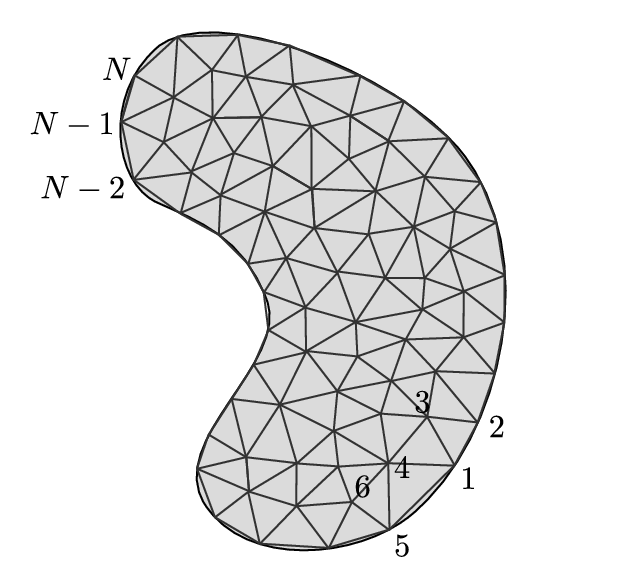
\includegraphics[width=0.45\textwidth]{papers/fem/images/2d_mesh.png}
    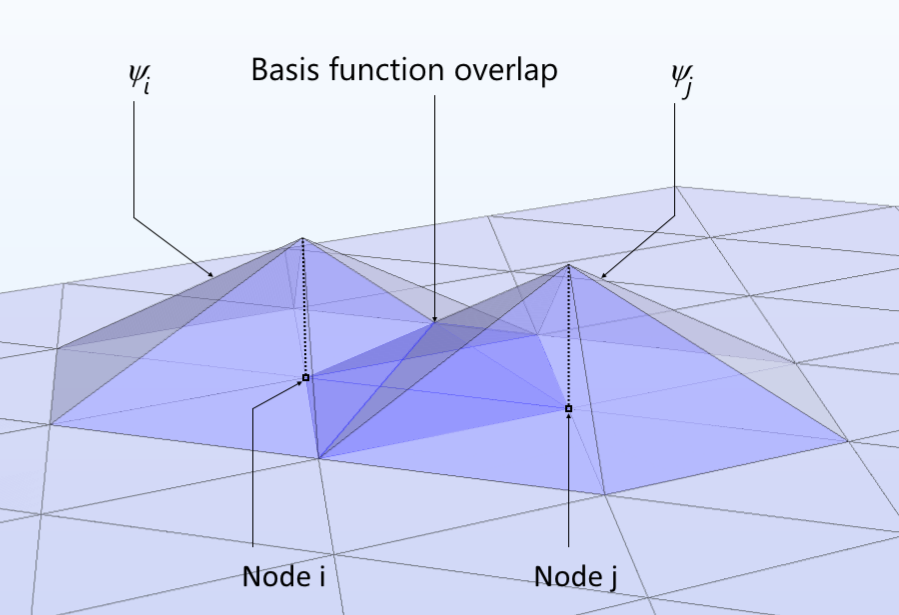
\includegraphics[width=0.45\textwidth]{papers/fem/images/2d_basisfkt.png}
    \caption{Der in dreieckige Elemente unterteilte Definitionsbereich mit nummerierten Knotenpunkten (links) und die linearen Basisfunktionen zweier Elemente, die sich berühren.}
    \label{fem:nd:2d_mesh_und_basisfkt}
    \end{figure}
    


\subsection{Erstellen der Matrix}
Das zu lösende Problem wird erneut diskretisiert, es werden also einzelne Punkte aus dem Definitionsbereich ausgewählt.
Diese Knoten werden dann jeweils mit den nächstgelegenen Nachbarn verbunden und nummeriert.
Bei der Nummerierung der Elemente sollte darauf geachtet werden, dass benachbarte Elemente auch in der Nummerierung nebeneinander sind, da so die Matrix ``möglichst diagonal'' wird.
Dies macht das Invertieren effizienter.
Es sollte ein Bild ähnlich des zweidimensionalen Beispiels in Abbildung \ref{fem:nd:2d_mesh_und_basisfkt}
resultieren.

Zum Befüllen der Matrizen wird analog zum eindimensionalen Fall jeder Eintrag mit der zugehörigen Formel ausgewertet.
Für $\mathbf{L}$ gilt
\begin{equation}
    l_{ij} = \int_{\Omega} \nabla a_i(\vec{x}) \cdot \nabla a_j(\vec{x}) \diff \vec{x},
\end{equation}
während für $\mathbf{M}$ 
\begin{equation}
    m_{ij} = \int_{\Omega} a_i(\vec{x}) \cdot a_j(\vec{x}) \diff \vec{x}
\end{equation}
eingesetzt werden muss.

Es werden auch hier nur die Einträge ungleich null sein, deren Elemente sich berühren.
Der Eintrag in der Zeile $a$ und Spalte $b$ ist also nur dann ungleich Null, wenn Element $a$ und Element $b$ im Graphen \ref{fem:nd:2d_mesh_und_basisfkt} verbunden sind.

\subsection{Codieren der Anfangsbedingungen}
Das Vorgehen zum Codieren der Anfangsbedingungen unterscheidet sich nicht von dem des eindimensionalen Falls. 
Dieses wurde in Kapitel \ref{fem:1d:anfangsbedingungen} behandelt.
TODO: Problem der Normal-Ableitung (-> PDE-Vorlesung).

\subsection{Invertieren der Matrix}
Auch hier unterscheidet sich das Vorgehen nicht vom im Kapitel \ref{fem:1d:matrix_invertieren} behandelten eindimensionalen Fall.